%\setchapterimage{fig_00.jpg}
\chapter*{Application \arabic{cptApplication} \\ 
Guidage linéaire de systèmes médicaux -- \ifprof Corrigé \else Sujet \fi}
\addcontentsline{toc}{section}{Application \arabic{cptApplication} : Guidage linéaire de systèmes médicaux -- \ifprof Corrigé \else Sujet \fi}

\iflivret \stepcounter{cptApplication} \else
\ifprof  \stepcounter{cptApplication} \else \fi
\fi

\setcounter{question}{0}

\marginnote[1cm]{Ressources de Renan Bonnard.}
\marginnote[1cm]{
%\UPSTIcompetence[2]{B2-14}
%\UPSTIcompetence[2]{C1-05}
%\UPSTIcompetence[2]{C2-07}
}



\begin{marginfigure}
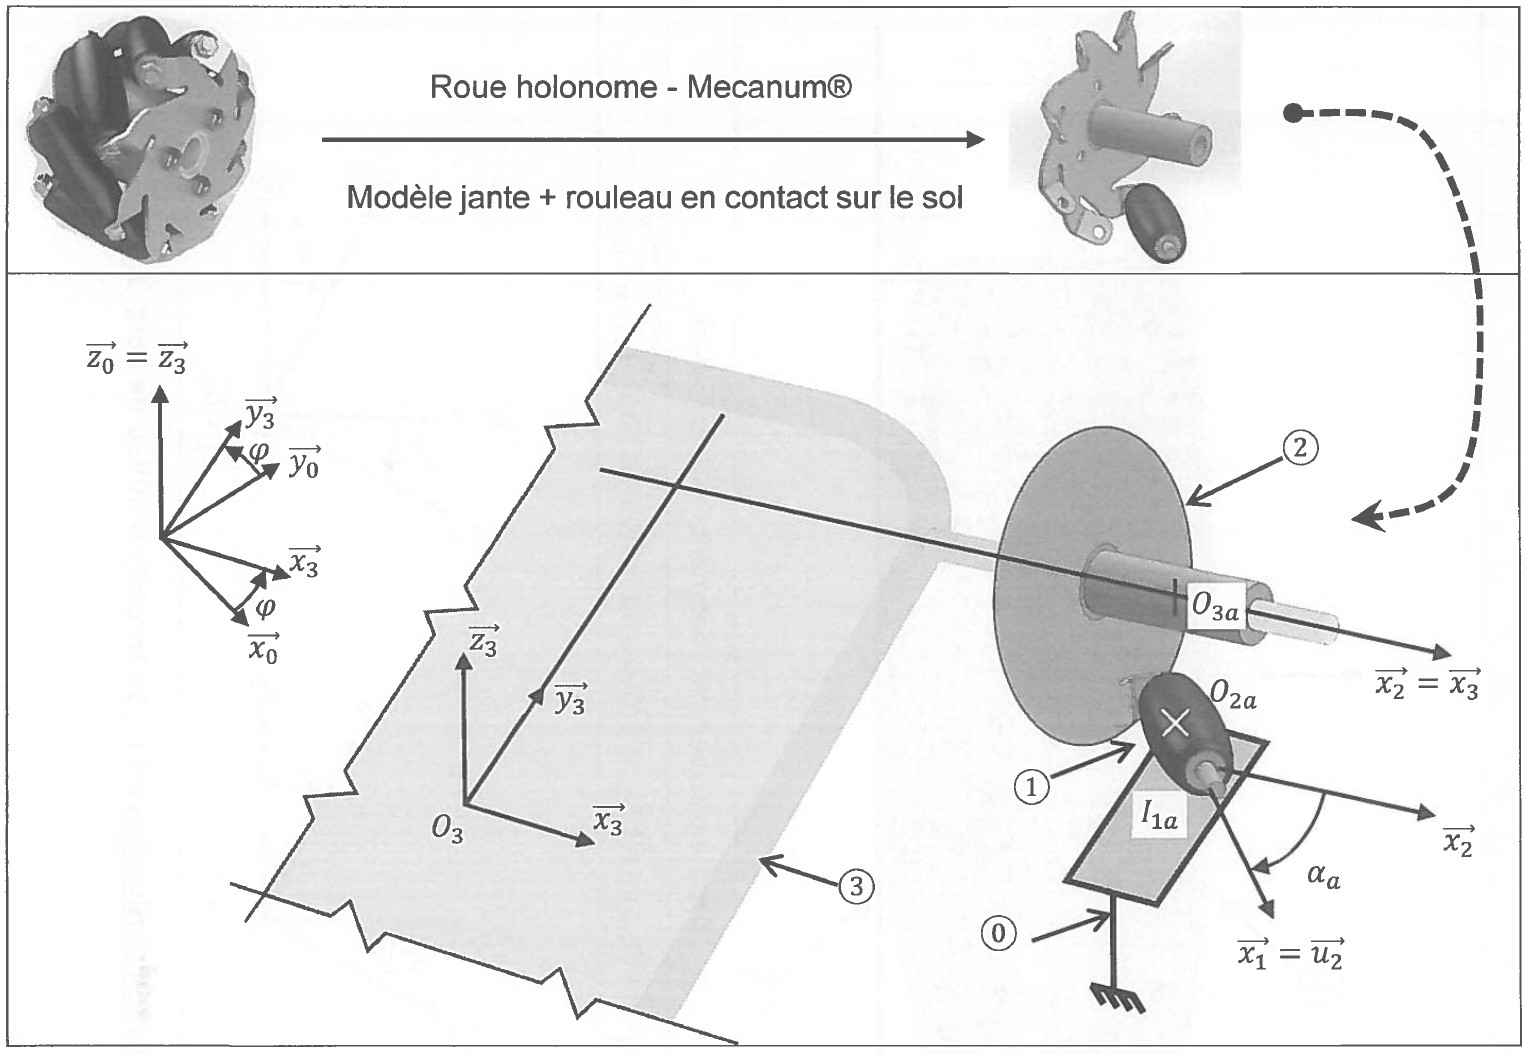
\includegraphics[width=\linewidth]{fig_04}
\end{marginfigure}

L’étude suivante porte sur le guidage en translation d’un chariot 
de scanner médical S1 par rapport au bâti de la machine S0. Ce 
guidage est réalisé par deux séries de billes, S2 et S3, qui roulent 
dans des rainures en V. 

La figure ci-dessous présente, en coupe, la réalisation technologique de ce guidage. 

\begin{center}
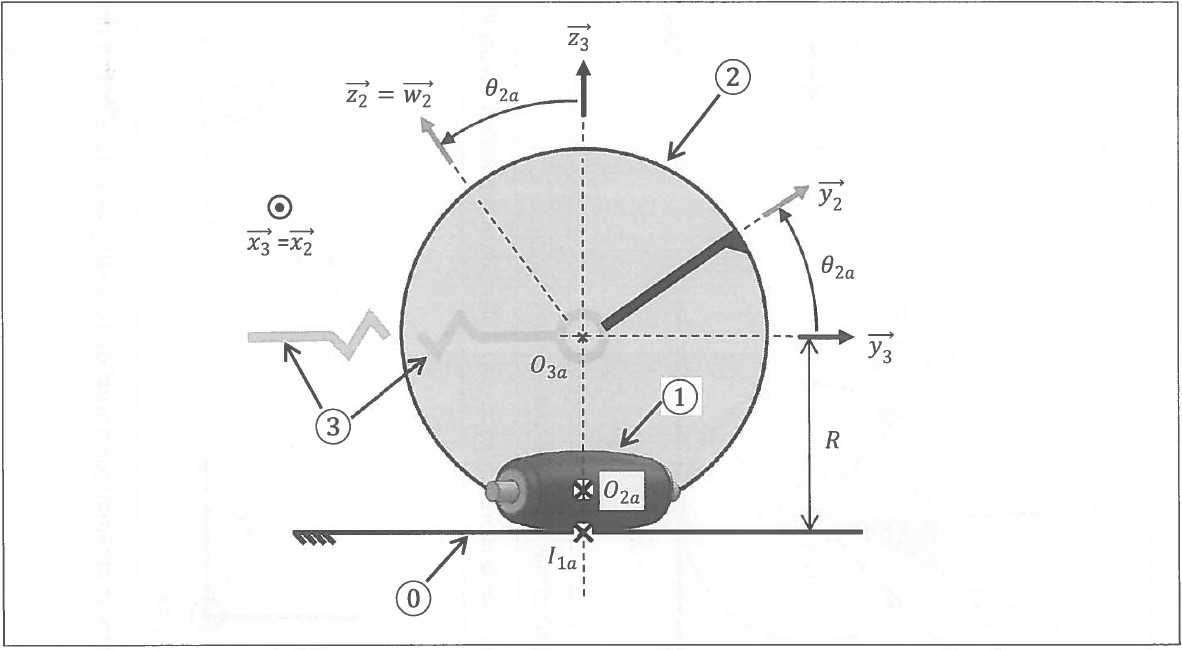
\includegraphics[width=\linewidth]{fig_05}
\end{center}

Les billes S2 de rayon $R$ roulent sans glisser sur les plans d’une rainure en V d’angle égal à 90\textdegree usinée dans 
S1 et sur les plans d’une autre rainure en V d’angle égal à 120\textdegree usinée dans S0. 
Les billes S3 de rayon $r$ roulent sans glisser sur les plans d’une rainure en V d’angle égal à 
$2\alpha$ usinée dans 
S1 et sur le plan (P) de S0. 

On note $\torseurcin{V}{1}{0}=\torseurl{\vect{0}}{v\vect{x}}{\forall P}$ le torseur cinématique du mouvement du chariot S1 par rapport au bâti S0. 

On pose $\vecto{2}{0} = \omega_{20}\vect{y}$ et $\vecto{3}{0} = \omega_{30}\vect{y}$.

\question{Traduire les conditions de non glissement. En déduire quelques axes instantanés de rotation.}
\ifprof
\begin{corrige}
\end{corrige} \else \fi

\question{Déterminer $\vectv{C}{2}{0}$ en fonction de $v$, puis $\vectv{E}{3}{0}$ en fonction de $v$. Déterminer $\vectv{C}{2}{0}$ en fonction de $\omega_{20}$, puis $\vectv{E}{3}{0}$ en fonction de $\omega_{30}$. En déduire une relation entre $\omega_{20}$ et $v$, puis une relation entre $\omega_{30}$ et $v$.}
\ifprof
\begin{corrige}
\end{corrige} \else \fi

\question{En déduire les torseurs cinématiques des mouvements de S2/S0 et S3/S0 en fonction de v et 
des caractéristiques géométriques.}
\ifprof
\begin{corrige}
\end{corrige} \else \fi

\question{Préciser les composantes de roulement et de pivotement en $G$ et $B$.}
\ifprof
\begin{corrige}
\end{corrige} \else \fi

\question{Déterminer les vecteurs vitesses des centres des billes dans leur mouvement par rapport au bâti S0 : $\vectv{O_2}{2}{0}$ et $\vectv{O_3}{3}{0}$.}
\ifprof
\begin{corrige}
\end{corrige} \else \fi

\question{Déterminer $\alpha$ pour que ces vecteurs vitesses soient identiques. }
\ifprof
\begin{corrige}
\end{corrige} \else \fi
